\chapter{Preliminary Studies}
\label{chap:Prelim}

This chapter describes the two week long initial phase of this project, from 28.08.2014 to 15.09.2014, which was used to create frameworks for both social and technical procedures. During this phase the project goal was defined and solutions were discussed. After deciding on a solution it was further conceptualized by creating use cases and functional requirements, as well as investigating the current market situation. The chapter includes an overview of what we did in this phase and also details the life cycle model used in this project.

\section{Work done this phase}
\label{sec:PrelimWork}
The preliminary studies phase started on 28.08.14 with the first meeting between the group and the customer. At this meeting the customer presented their idea of a service which would serve as a virtual city space and enable youth to share mediated expressions. At the time of the meeting the customer only had an abstract idea of the service, with few a concrete features they wanted and no preferred approach to deliver these features, the tasks of creating a design through which the services would be provided was left to the group. The tasks to be completed in the project specified in this meeting are[customer - 28.08.14]:
\begin{itemize}
  \item To design a new platform experience that can facilitate digital sharing of mediated expressions across urban communities globally.
  \item A commercial-free digital hub where youth can upload, share and create content.
  \item Strengthening their local engagement, expression of ideas and experimental thinking.
  \item increase youth participation and political influence on the development of city spaces.
\end{itemize}

\begin{figure}[ht!]
  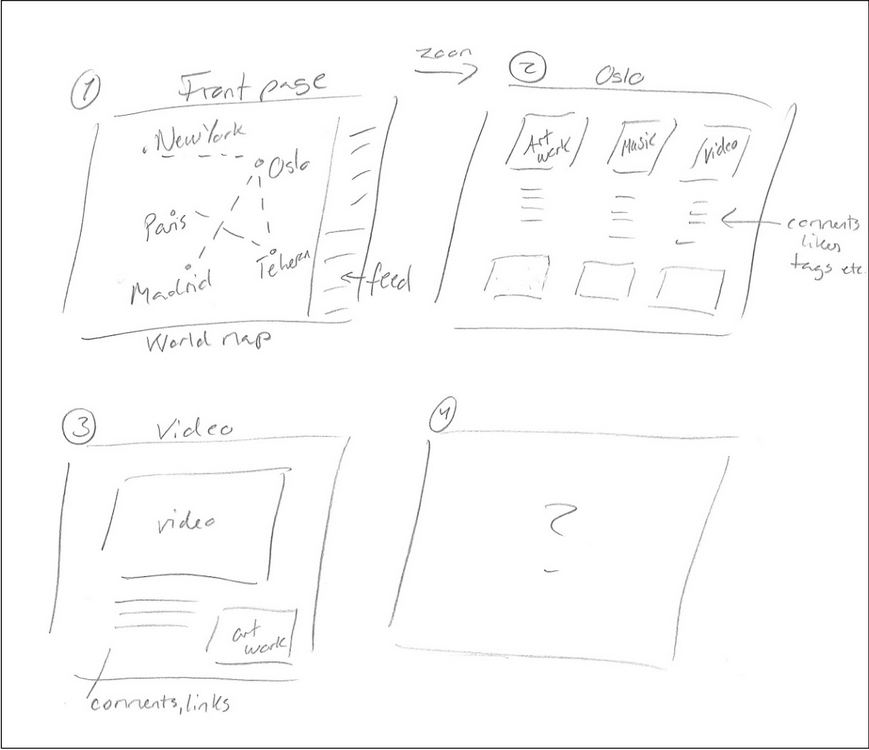
\includegraphics[width=\linewidth]{./PreliminaryStudies/img/conceptSketch}
  \caption{Original concept sketch by AFI}
  \label{fig:PrelimWorkSketch}
\end{figure}

Following this meeting the group had several meetings where different ideas were considered and discussed. During the two weeks in this initial phase the group had group meetings or other compulsory team activities five days a week. The frequent meetings were crucial in ensuring that the group thoroughly discussed all ideas and arrived at a concept without large disagreements or misunderstandings.
\paragraph{} By the end of the first week a core concept was conceived detailing the necessary functions for a web application. An initial demo was made combining some of these functions with the basic design idea the customer had presented on the initial meeting. During the second week of this phase the group decided how to solve some of the technical issues relating to the basic design of the service, and preliminary studies of the target market were begun. The results of the initial market investigations are included at the end of the chapter, even though the finishing touches were done at the start of the first sprint.

\subsection{Concretizing and narrowing down the project}
\label{subsec:PrelimWorkConcret}

In order to make a concrete set of requirements detailing the core functionalities of the system, an initial set of use cases were made, representing the initial actions the group would want to be able to make with a service like the one described by the customer. After making this set of use cases the customer was asked to prioritize them to further enable proper work distribution on the project. These initial use cases were:

\begin{enumerate}
  \item Searching for locations and pictures (based on tags).
  \item Uploading pictures.
  \item Creating and joining events.
  \item Adding new places and interests.
  \item Communicating directly with other people.
  \item Commenting on pictures
\end{enumerate}

The use cases were also used to specify the first draft of the system requirements. By applying the use case based project estimation process to these use cases we end up with an estimate of about 800 person hours of coding to complete all the functions.
\paragraph{} By the end of the first week a demo was developed to illustrate the basic functions, this demo used a map on which arrangements were displayed as small icons which could be clicked to expand a sidebar with further information about the event. The events were classified as belonging to an interest and could be filtered these interests by using of a search bar.
\paragraph{} Other features were also considered but were decided against for different reasons, see the further work sections for a comprehensive list of features that we think should be included in future versions. The customer suggested a streaming feature for sharing live shows and other arrangements, however due to the limited time frame of the project the livestream feature was postponed to a future version as it would require too much time and thus degrade the quality of the core features of the system.

\subsection{Project choices}
\label{subsec:PrelimWorkChoices}

During this first phase many decisions had to be made regarding the overall design of the project. Among other things the platform to be focused on had to be decided and cleared with the group. The initial presentation stated participation as a goal and the illustration of the idea was as a web page. As a web page is available through all modern browsers and can be accessed from all computers with an internet connection, while a mobile application is limited to a specific operating system and can not be accessed from a computer the group decided to focus on a web page interface in the limited time frame of the project.


\subsubsection{Location management}
A more technical choice of solution occurred in regards to how places were managed in the system, two different models were considered as solutions to this problem. One model uses pre-generated locations, like club houses, cafes, or parks as a basis for where content can be located, this model was dubbed the Location model. For instance a football match would be located at a defined football field, while a concert might be located at a bar.

\subsubsection{Location model}
This offers the advantage of enabling a compact view of events organized at a specific location. Unfortunately this approach also creates problems, especially when content originates in locations that are not managed by one or more people. This model makes it hard to place content generated at some street corner, or in a person's home. Furthermore generating all these locations is a time consuming task that requires specialized knowledge of the area in question. A solution to this problem is to delegate this task to users of the system, but that creates other problems related to the creation of a duplicate location. If there are two separate locations in the system that both have information relating to the same real world location, a user can only view the information on one of the virtual locations at a time. This causes the display of faulty and incomplete information on the site. A way of combating this is to hire one or more people to manage and merge duplicated locations, this incurs the additional cost of paying these workers.


\subsubsection{Proximity model}
The alternative solution was dubbed the Proximity model. This model manages content based on coordinates instead of locations. Because all content is placed at an exact location it does require a certain level of ability to use maps in order to navigate the site and search for content. If the search area is too specific some results might be outside the search, for instance if looking for pictures from a football match and zooming in to cover only half the field some content might have been placed in the other half. This approach is well suited for combination with a mobile application with GPS functionality for automatic placement. After considering both solutions and counseling the customer[customer 12.09.14] the Proximity model was chosen for the project.

\section{Market Investigation}
\label{sec:PrelimMarket}

The following section looks at existing products that may be used as a solution to some or all of the problems Alternative Spaces is intended to solve.

\subsection{Current situation}
\label{subsec:PrelimMarketSituation}
As of today there are many social networks and young people are avid users of several of these. However, a lot of networks that are most popular with young people are focused mostly on connecting with people you already know or at least are acquainted with. Even as this makes them excellent for maintaining established social relations, it makes them less useful as arenas for meeting new people and finding new interests.

\paragraph{} As a solution to this problem the site \href{http://www.meetup.com}{meetup.com} offers a service where users can make events, classify the events as matching some interest and then other users can attend those events. However this alternative is only available for users over 18 years old, and is furthermore populated in large part by a computer focused demographic.

\paragraph{} The customer has stated that one goal of the project is to “increase youth participation and political influence on the development of city spaces”. In regards to this, while most political parties are represented on several social media these mostly serve as a one-way communication channel from the politicians to the masses, rather than as a place where they listen. This is unfortunately difficult to change, even with a new social network, since it requires the right mindset from the politicians in question, but if such a mindset exists, social media can be designed to better facilitate such an exchange of ideas.

\subsection{Desired situation}
\label{subsec:PrelimMarketDesired}

In the future our platform will serve as a forum for youth all over the world to connect and find new friends and interests, browse and share media related to their interests, organize and join events, and also as a channel for youth to express their political opinions in a place where they can be seen by local politicians.

\subsection{Competitors}
\label{subsec:PrelimMarketCompetitors}

\begin{itemize}
  \item \textbf{Facebook} has extensive functionality for connecting with friends and creating events and groups for a selection of these. This makes Facebook the natural next step after using our system, meet new people on Alternative Spaces and stay connected with them on Facebook. \begin{itemize}
    \item Users already have a large existing Facebook network
    \item Most people are users already
    \item Using Facebook mostly for the chatting and messaging service seems to be a trend amongst young people, and we should look into this and decide if we want that functionality
  \end{itemize}
  \item \textbf{Twitter} provides the possibility of advertising events, but a lack of functionality for opting in or attending events makes it impractical.
  \item \textbf{Reddit}  is great at making communities centered around any more or less specific interest. Making subreddits for certain interests is a way to organize and advertise events, and the subreddit could serve as a channel to discuss relevant interests. However, based on research from the U.S. only a fairly small amount, about 4\%, of Reddit users are under the age of 18, making it a less useful channel for reaching this group. Also, finding subreddits for location specific interests might be hard.
  \item \textbf{Meetup} offers much of the same event organization and finding as we plan to implement. They let users define searches through interests as well as location, using both cities or postal code combined with an adjustable radius to limit the search area. \begin{itemize}
    \item Meetup requires users to be at least 18 years old, which does not make them a direct competitor to us.
    \item Meetup appears to have a largely IT focused userbase judging from meetups in Oslo and Trondheim.
  \end{itemize}
\end{itemize}

\subsection{Generating Revenue}
\label{subsec:PrelimMarketRevenue}
Depending on the system's need to generate income some models may be considered.
\begin{itemize}
  \item \textbf{Freemium:} Some functions available for free while others are exclusive for users that have payed for a premium account.
  \item \textbf{Subscription:} Offer several different levels of payment and increase utility as price rises.
  \item \textbf{Advertising:} This seems like the least wanted solution from the customer's point of view.
  \item Depending on the system and the events getting organised, the users can buy the tickets for the events they are interested in.
\end{itemize}

Considering that the stated purpose of the system was to help youth in an increasingly commercialized city space, we decided to scrap looking further into how to generate revenue.

\section{Life Cycle Model}
\label{sec:PrelimMethod}

This section deals with the two different life cycle models considered for this project. The first is the Waterfall model and the second is the Scrum model. To compare these two completely different methods it is necessary to analyze both with regards to the project. For this reason the main idea of both models will be presented and the advantages and disadvantages of each will be mentioned. After this there will be a conclusion as to which model is better suited to this project and will be used. There will be also an explanation why this model was chosen.

\subsection{The Waterfall model}
\label{sec:PrelimMethodWaterfall}
The first model that was analyzed was the Waterfall model. It demonstrates the linear flow of the software development cycle. In this model any given phase can only start when the previous phase was finished, like a Waterfall. The reason for this is that the output of the previous phase in general represents the input to the next phase. Figure \ref{fig:PrelimMethodWaterfall} illustrates the Waterfall model.

\begin{figure}[ht!]
  \centering
  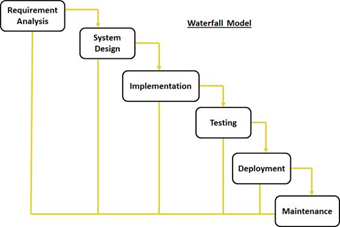
\includegraphics[width=80mm]{./PreliminaryStudies/img/waterfall}
  \caption{The Waterfall lifecycle}
  \label{fig:PrelimMethodWaterfall}
\end{figure}

\paragraph{}The first phase is requirement analysis. In this stage the goal is to collect and document all possible requirements of the system in a requirement specification document. The next phase uses this document to prepare the system design. For example, creating use cases and specifying hardware and system requirements. The main goal of the third phase is implementing the functionalities that were designed in the second stage. In the testing phase every unit is tested to try to find errors and problems in the program and fix them. It is the last step before the product will be released on the market. In the deployment phase, the finished product is released. The last stage, maintenance, consists fixing issues that come up in the client environment like bugs that were not detected in the testing phase.

\subsubsection{Advantages}
The Waterfall model with it sequential approach, is really easy to understand and to use. The processing and completing of every phase is at one time. The stages are clearly defined and also every stage has concrete deliverables. The whole process and every phase are very well documented, because it is needed for starting the next stage. Additionally it is easy to organize tasks.

\subsubsection{Disadvantages}
The sequential approach of Waterfall model does not only lead to advantages but also disadvantages. This model is not good for complex projects and especially not long projects, because the result are seen very late when changes are very difficult to implement. With the Waterfall approach there is no working software before the whole project is finished.  Interaction with the customer is at predetermined times, and there is no prototype to show off ideas to them. When the customer arrives with changes, the only real choice is restarting at the fist phase or rejecting the new requirements.


\subsection{Scrum}
\label{subsec:PrelimMethodScrum}

A Scrum project has three different main roles. The first is the product owner, who delivers the vision for project. In most of the project the product owner is the customer. The second role is the Scrum master. He is responsible for supporting team work and finding solutions to conflicts. The Scrum team form the last role. It is responsible for the implementation of the project and at the end delivering a completed product.

\paragraph{} At the beginning of a Scrum project the first step is to create a product backlog. This backlog consists of all requirements that should be fulfilled in the final product. Unlike the Waterfall model Scrum is focused on delivering a working prototype as soon as possible. That means that Scrum projects consist of many iterations, so called Sprints, where each Sprint contains the same stages as the Waterfall model with its own small product and its own requirements as shown in figure \ref{fig:PrelimMethodScrumIter}.

\begin{figure}[ht!]
  \centering
  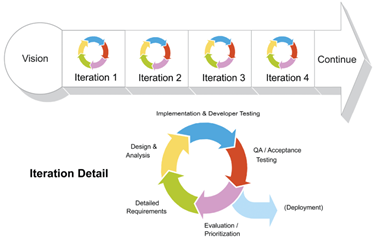
\includegraphics[width=90mm]{./PreliminaryStudies/img/scrum}
  \caption{The iterative approach of Scrum}
  \label{fig:PrelimMethodScrumIter}
\end{figure}

\paragraph{} Every sprint starts with a planning meeting. In this meeting the Scrum team has to decide which product requirements they wish to work on in this sprint. The goal is to make a sprint backlog which includes only part of the product backlog. The important part is that the sprint backlog cannot be changed during the sprint, and all requirements on the backlog need to be completed. To make sure the implementation is on time, there is a daily Scrum meeting. At this meeting, every member of the team has to answer the following questions:

\begin{itemize}
  \item What have you done since the last meeting?
  \item What will you do until next meeting?
  \item What problems did you have?
\end{itemize}

\paragraph{} This information makes it easier to get a good overview of the status of the project. A sprint normally lasts between two and four weeks as shown in figure \ref{fig:PrelimMethodScrumLife}.

\begin{figure}[ht!]
  \centering
  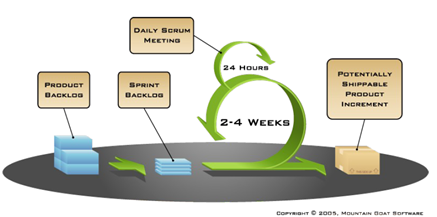
\includegraphics[width=100mm]{./PreliminaryStudies/img/scrum2.png}
  \caption{The Scrum lifecycle}
  \label{fig:PrelimMethodScrumLife}
\end{figure}

\paragraph{} At the end of every sprint the output is a working product, with the features of the sprint requirements. Each sprint ends with a review meeting in which the Scrum team presented the product and a retrospective meeting. This meeting is a way of lesson learned. This means that there will be a discussion about the good and bad things of this sprint and also the things that can be improved in the next sprint.

\subsubsection{Advantages}
Delivering a working project after each sprint is one of the big advantages of Scrum, because the status of the project can be seen after each sprint. With this approach the team can easily abort or change the scope or direction of the project, because the requirements are not fixed variables. Another advantage is that the customer has more possibilities to participate in observing and changing the final result, because they can often see parts of the final product. This makes it easier to get feedback early. Another advantage is that the daily meetings in Scrum help to measure the productivity of each person.

\subsubsection{Disadvantages}
The freedom of changing the scope and also the freedom of working is not always an advantage. When the tasks that have to be done are not defined exactly, the estimation of cost and time can be wrong and spread over more than one sprint. Another thing is that the Scrum master who manages the group has to trust his project members otherwise with too much control the team members can get frustrated. A missing commitment in team members leads to the project never completing.

\section{Choice of Life Cycle Model}
%TODO RECHECK PHRASING
After analyzing these models, it was clear that both had their strengths and weaknesses. The customer's vision of this project was as part of a research project. The requirements for the prototype were not described in detail, nor fixed, and making choices would be a large part of the project. Because of this, we needed to choose a model where changes were easy to handle. The product is going to be used by youth, and usability for this group is important. The customer also arranged for the possibility to get feedback from end users, but only midway through development, which meant that we could not use a model that had all requirements set in stone at that point. This also meant we needed something to show off at that point to get good feedback. This meant that the Waterfall model was not suited for our needs, while Scrum gave us all of these. Because of this we chose Scrum as our choice for lifecycle model.